% 2008 年江苏卷第 21A 题：△ABC 的外接圆，切线 AE 与 BC 延长线交于 E，AD 平分 ∠BAC。
% 来源 PDF：gaokaomath-src/普通高考/2008/2008江苏.pdf
% SHA-256：b998b93963143559a1ce800a6d320de618883b0e22ee5130b7666a2374caeba0
% 原页：2008江苏.pdf 第 2 页（A3 三栏）第 2 栏，书页码 458。
% 绘制依据：按原页画圆、圆上 A（上）、B（左上）、C（右下），BC 延长线上的 E，
%   切线 AE，以及 ∠BAC 的平分线 AD（D 在 BC 上）。
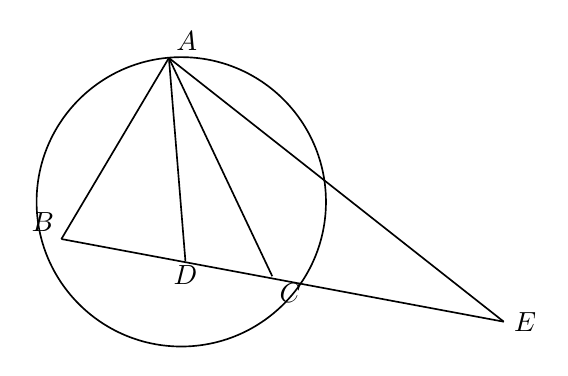
\begin{tikzpicture}[scale=1.05, semithick, every node/.style={inner sep=1.4pt}]
  % 外接圆
  \draw (2.2,1.5) circle [radius=1.75];

  \coordinate (A) at (2.05,3.24);
  \coordinate (B) at (0.75,1.05);
  \coordinate (C) at (3.30,0.60);
  \coordinate (D) at (2.25,0.78);
  \coordinate (E) at (6.10,0.05);

  \draw (B) -- (E);
  \draw (A) -- (B);
  \draw (A) -- (C);
  \draw (A) -- (E);
  \draw (A) -- (D);

  \node[above right=1pt] at (A) {$A$};
  \node[above left=1pt] at (B) {$B$};
  \node[below right=1pt] at (C) {$C$};
  \node[below] at (D) {$D$};
  \node[right=2pt] at (E) {$E$};
\end{tikzpicture}
